\section{Theorie}
Die Anwendung von Brückenschaltungen liegt in der Messtechnik,  vorallem von Wiederständen. 
Hier sollen sie durch eine Nullmethode die Auflösung der Messsung erhöhen um so präzisere Ergebnise
auslesen zu können. Dadurch lassen sich nicht nur reele wie komplexe Wiederstände, sondern auch eben 
solche Daten messen die den Wiederstand beeinflussen, wie zum Beispiel Temperatur oder Längenänderung. %ist das der grund?
Die Funktionsart eine Brückenschaltung beschränkt sich im wesentlichen auf die Abtastung einer 
Potentialdifferenz zwischen zwei Punkten. 
\begin{figure}
    \centering
    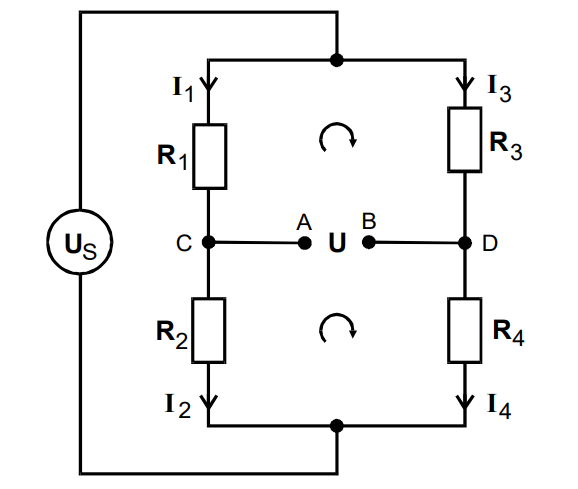
\includegraphics[width=0.1\textwidth]{bilder/abb1.png}
    \caption{Allgemeines Schema einer Brückenschaltung. \cite{skript}} 
    \label{fig:abb1}
\end{figure}
Diese Differenz der Spannung $U_Bs$ wird im allgemeinen Brückenspannung genannt und zwischen den Punkten $A$ und $B$ gemessen.
\\
\newline



\subsection{Kirchhoff'schen Gesetze}
Zentrale Grundlage der Berechnung sind die sogenannten Kirchhoff'schen Gesetze. Diese sind zweigeteilt und 
geben Auskumpft über den fließenden Strom in einem geschlossenen Kreis.
Das erste Gesetz besagt, dass in einem Knoten, also in einem Ort in dem der Strom zusammen - oder auseinander fließt, 
die Summe von elektrischen Strömen gleich Null ist.
\begin{equation}
    \sum_k \text{I}_k = 0
\end{equation}
Das zweite Gesetzt erläutert den Erhalt des fließenden Stroms, so dass in jedem abgeschlossenen Stromkreis, also einer Masche,
die Summe aller Teilspannungen gleich Null ist.
\begin{equation}
    \label{eqn:kirch2}
    \sum_k \text{U}_k = 0
\end{equation}
\begin{figure}
    \centering
    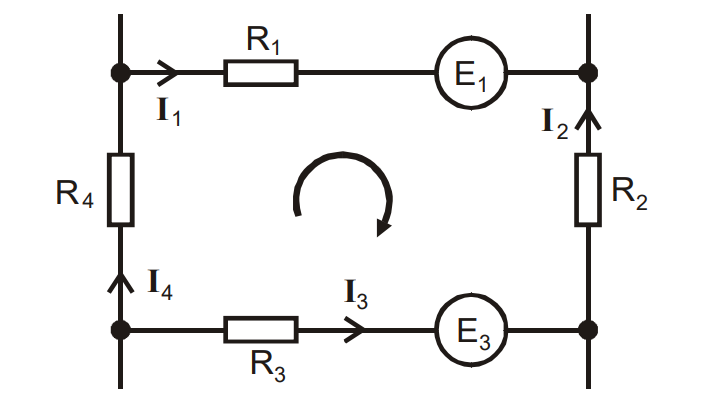
\includegraphics[width=0.6\textwidth]{bilder/abb3.png}
    \caption{Beispiel einer Masche in einem Schaltplan. \cite{skript}} 
    \label{fig:abb3}
\end{figure}
Die Spannung U aus der Gleichung ist ein Produkt aus dem Strom und den von diesem erfahrenen Wiederstand.
\begin{equation}
    \text{U} = \text{R}\cdot \text{I}
\end{equation}
Unter Anwendung dieser Gesetze auf den Schaltplan %ref auf fig abb1
lässt sich der folgene Zusammenhang finden. Hier bezeichnet $U_s$ die vom Generator erezugte Spannung, also die Speisespannung. 
\begin{equation}
     U= \frac{R_2R_3 - R_1R_4}{(R_3+R_4)(R_1+R_2)}\cdot U_s
\end{equation}
Sollte die Brückenspannung verschwinden liegt eine sogenante abgeglichene Brücke da. 
Hieraus lassen sich also die Werte für unekannten Widerständen in diesem Stromkreis finden.
Die Bedingung dafür ist.
\begin{equation}
    \label{eqn:bedingung}
    R_1 R_4 = R_2 R_3
\end{equation}
\\
\newline
\subsection{komplexe Widerstände}
Wenn ein Widerstand von einem Kondensator oder durch Induktivität erzeugt wird, ist dieser nicht mehr reines 
Element der reellen Zahlen. 
Die jetzt zum Teil komplexe Darstellung setzt sich aus dem reellen Teil des Wirkwiderstandes $X$ mit 
dem imaginären Blindwiederstand $Y$ zusammen. 
\begin{align*}
    R &= X +iY \\
    \Re{R} &= X \\
    \Im{R} &= Y 
\end{align*} 
Hier liegen also pro Widerstand zwei Paramter vor. Nach der Bedingung \eqref{eqn:bedingung} müssen also
nun der reelee und der imaginäre Teil übereinstimmen. 
\\
\newline
\subsection{Wheatstonesche Brückenschaltung}
\begin{figure}
    \centering
    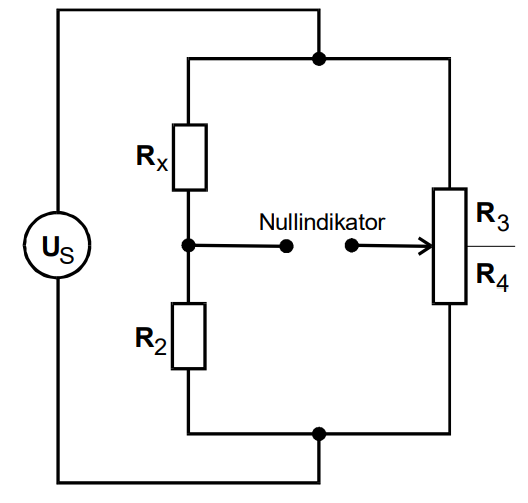
\includegraphics[width=0.3\textwidth]{bilder/abb4.png}
    \caption{Schaltplan einer Wheatstoneschen Brückenschaltung. \cite{skript}} 
    \label{fig:abb4}
\end{figure}
Bei der Wheatstoneschen Brückenschaltung gibt es ausschließlich reelle Wiederstände, also  keine Kondensatoren
oder Induktivitäten. Daraus folgt, dass die angelegte Spannung keine Rolle spielt. Es kann also frei zwischen
Gleich - und Wechselstrom gewählt werden. Aus der Abgleichbedingung \eqref{eqn:bedingung} folgt.
\begin{equation}
    R_x = R_2 \frac{R_3}{R_4}
\end{equation}
\\
\newline
\subsection{Kapazitätsmessbrücke}
\begin{figure}
    \centering
    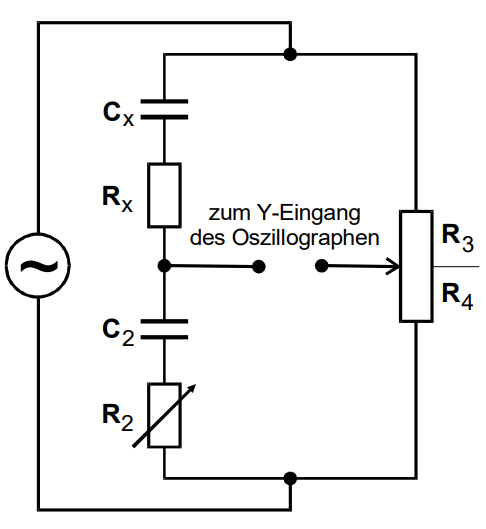
\includegraphics[width=0.3\textwidth]{bilder/abb6.png}
    \caption{Schaltplan einer Kapazitätsmessbrücke mit dielektrischen Verlusten. \cite{skript}} 
    \label{fig:abb6}
\end{figure}
Bei realen Kodensatoren kann nicht gewährleistet werden den Strom ohne Verluste ,zum Beispiel Wärme, 
zu konservieren. Es eignet sich also dem Schaltplan einen Wiederstand hinzuzufügen der für die Verluste aufkommt.
Mit einführung des Kondensators $C_x$ erweitert sich der Widerstand um einen komplexen Anteil der bei der Messung durch 
einen zweiten, veränderlichen Widerstand kompensiert wird. 
Es folgt aus \eqref{eqn:bedingung}.
\begin{align}
    R_x &= R_2\frac{R_3}{R_4} \\
    C_x &= C_2\frac{R_4}{R_3}
\end{align}
\\
\newline
\subsection{Induktivitäts - und Maxwellbrücke }

\begin{figure}
\begin{minipage}[c]{0.5\textwidth}
    \centering
    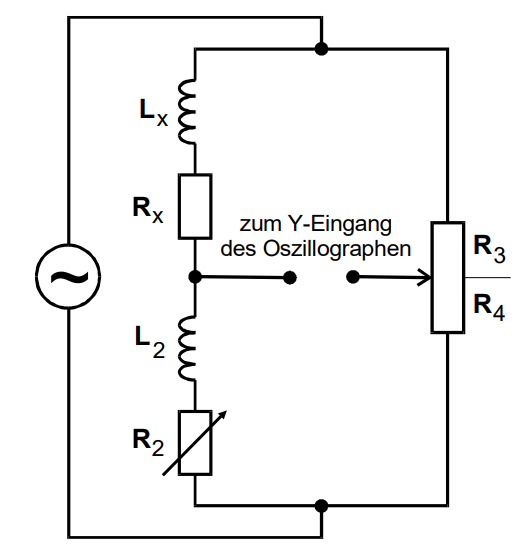
\includegraphics[width=0.7\textwidth]{bilder/abb8.png}
    %\caption{Schaltplan einer Induktivitätsbrücke. \cite{skript}} 
    \label{fig:abb8}
\end{minipage}    
\begin{minipage}[c]{0.5\textwidth}
            \centering
        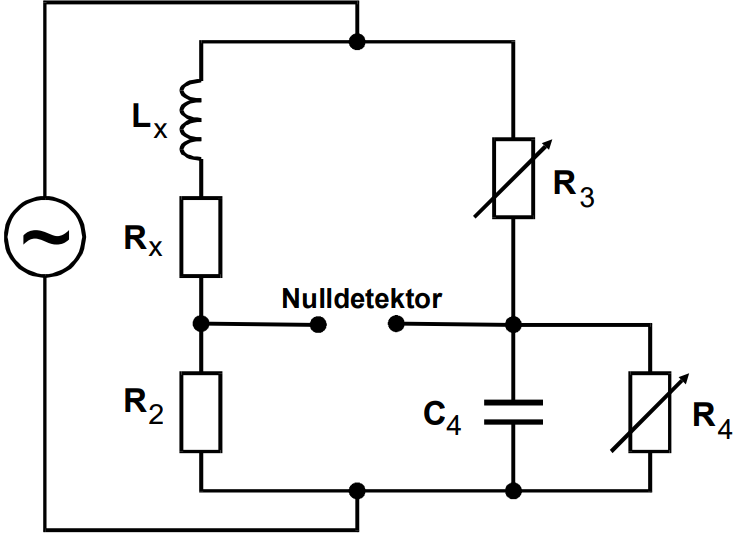
\includegraphics[width=\textwidth]{bilder/abb9.png}
        %{0.5\textwidth}
        \label{fig:abb9}
\end{minipage}
\caption{Schaltplan einer Induktivitäts - und Maxwellbrücke. \cite{skript}}
\end{figure}


Analog zum Kondensator gelingt es auch bei realer Induktivität nicht den Strom verlustfrei weiterzuleiten.
Als Beiprodukt entsteht durch magnetische Feldenergie Wärme, was als fiktiver Widerstand in den Schaltplan einzeichnet wird.
Um die Induktivität $L_x$selbst zu bestimmen wird eine Spule mit bekannten Werten der Schaltung hinzugefügt. 
Ähnlich zur Kondensatorbrücke lässt sich der gesuchte Wiederstand und die Induktivität wie folgt finden.
\begin{align}
    R_x &= R_2\frac{R_3}{R_4} \\
    L_x &= L_2\frac{R_3}{R_4}
\end{align}

Um den Verlusten der Induktivität von $L_2$ entgegen zuwirken bietet es sich an diese durch eine Kondensator $C_4$ mit bekannten Werten
zu wechseln. Die Konfiguartion der Brückenschaltung nennt sich Maxwellbrücke.
%include abb9
Dadurch rezuziert sich der Wikrungswiederstand und die Bestimmung von $L_x$ wird präziser.
\begin{align}
    R_x &= R_2\frac{R_3}{R_4} \\
    L_x &= R_2R_3C_4
\end{align}
\\
\newline
\subsection{Wien-Robinsonbrücke}
\begin{figure}
    \centering
    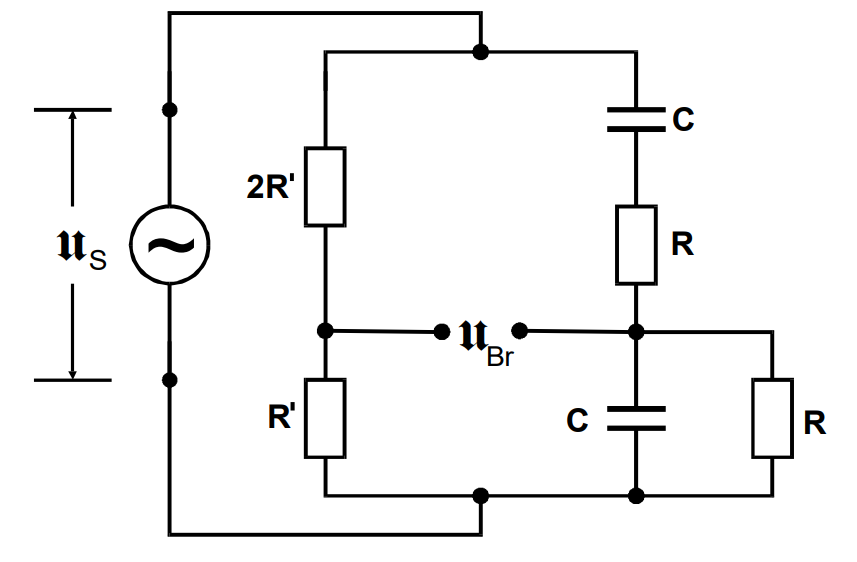
\includegraphics[width=0.3\textwidth]{bilder/abb10.png}
    \caption{Schaltplan einer Wien-Robinsonbrücke. \cite{skript}} 
    \label{fig:abb10}
\end{figure}
Bei der Wien - Robinsonbrücke wird auf Abgleichelemente verzichtet und stattdessen mit einer variablen Frequenz gemessen.
Als Ergebnis folgt eine Brückenspannung die folglich abhängig von der Frequenz $\omega$ ist.
Werden die Widerstandsoperatoren der jeweiligen Elemente 
in die Bedingung für einen abgeglichen Zustand \eqref{eqn:bedingung} eingesetzt wird folgende Glecihung gefunden.
\begin{equation} % muss noch größere klammern abs()
    \label{eqn:bigBoi}
    {\biggl| \frac{U_{br}}{U_s} \biggr| }^2 = \frac{(\omega ^2 R^2 C^2 -1)^2}{9\Bigl[(1-\omega ^2 R^2 C^2)^2 + 9 \omega ^2 R^2 C^2 \Bigr]}
\end{equation}
Wenn nun also die Spannung $\frac{U_{br}}{U_s}$ verschwinden soll muss der Zähle eben Null werden. Das Bedeutet, dass für 
$\omega_0$ folgenes gelten muss.
\begin{equation*}
    \omega_0 = \frac{1}{RC}
\end{equation*}
Die Wien-Robinsonbrücke filtert also bestimmte Frequenz die sich Nahe bei $\omega_0$ befinden. Das Verhältnis wird definiert als.
\begin{equation}
    \label{eqn:OMEGALULW}
    \Omega = \frac{\omega}{\omega_0}
\end{equation}
Angewandt auf \eqref{eqn:bigBoi} wird folgene Gleichung gefunden.
\begin{equation}

    {\biggl| \frac{U_{br}}{U_s} \biggr| }^2 = \frac{1}{9}\frac{(\Omega^2 -1)^2}{(1-\Omega^2)^2+9\Omega^2}
\end{equation}
\\
\newline
\subsection{TT - Brücke}
\begin{figure}
    \centering
    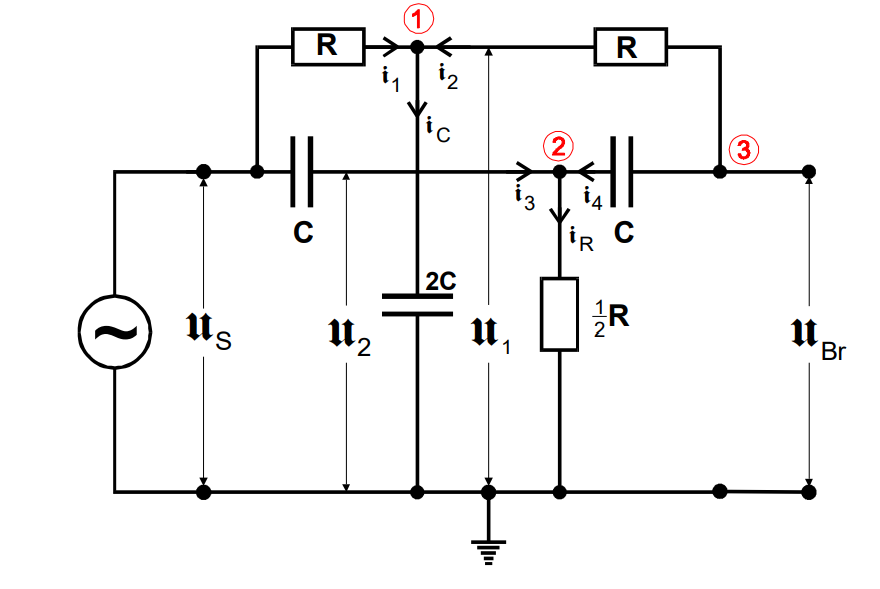
\includegraphics[width=0.3\textwidth]{bilder/abb11.png}
    \caption{Schaltplan einer TT - Brücke. \cite{skript}} 
    \label{fig:abb11}
\end{figure}
Wie auch schon die Wien-Robinsonbrücke funktioniert die TT - Brücke als Filter mit dem Unterschied, dass sowohl Eingangsspannung
$U_s$ als auch die Brückenspannung $U_{br}$ gegen Massen angeschlossen sind.
Mit dem gleichen $\Omega$ wie in \eqref{eqn:OMEGALULW} findet sich das Verhältnis von Brücken - zu Eingangsspannung.
\begin{equation}
    {\biggl| \frac{U_{br}}{U_s} \biggr| }^2 = \frac{1}{9}\frac{(\Omega^2 -1)^2}{(1-\Omega^2)^2+16\Omega^2} 
\end{equation}
\\
\newline
\subsection{Klirrfaktor}
Der Klirrfaktor beschreibt das Verhältnis zwischen dem Anteil einer, oft unerwünschten, Oberwelle im Verhältnis zu seiner Grundwelle.
Dieser Faktor gibt Auskunft über die Qualtität von meist Sinusgeneratoren und kann durch eine Wien - Robinsonbrücke ermittelt werden.
Ausgedrückt wird der Faktor durch.
\begin{equation}
    \label{eqn:GlasGoesklirr}   
    k = \frac{\sqrt{U_2^2+U_3^3+...}}{U_1}
\end{equation}
Die Amplituden der verschiedenen Oberwellen werden als $U_n$ angegebn wobei $U_1$ die Amplitude der Grundwelle beschreibt.














%\subsecton{Kirchhoffscheregel} %cSheck title,
%\subsection{komplexe wiederstände}
%\subsection{wheatstone}
%\subsection{kapazitätbrücke}
%\subsection{Induktivitätsbrücke}
%\subsection{maxwellBrücke}
%\subsection{wienrobinson}
%\subsection{TT-Brücke}